\documentclass[11pt]{article}
\usepackage{geometry}
\usepackage{graphicx}
\usepackage{enumitem}
\usepackage{float}
\usepackage{amsmath}
\usepackage{multicol}
\usepackage{cancel}
\usepackage{mathrsfs}

\geometry{a4paper, top=0.5in, bottom=0.5in, right=0.75in, left=0.75in}

\title{Lecture 8}
\author{}
\date{}

\begin{document}

\maketitle

\section{Frequency Pulling (Chirping)}

From CEO model:
\begin{align*}
    \chi' = \frac{2(\nu - \nu_o)}{\Delta \nu} \chi''
\end{align*}
In the presence of both host \& transition materials:
\begin{align*}
    n = \sqrt{\epsilon_r} = \sqrt{n_h^2 + \chi} = n_h \sqrt{1 + \frac{\chi' +j \chi''}{n_h^2}} \approx n_h + \frac{\chi'}{2n_h} + j \frac{\chi''}{2n_h}
\end{align*}
\textbf{Notes:}
\begin{itemize}
    \item The transition material's $\chi$ affects both the real and imaginary parts of the refractive index (n).
    \item Changing the imaginary part was intended in order to obtain a gain medium. However, the change in real part causes Chirping.  
\end{itemize}
\begin{align*}
    e^{-jnk_o z} = e^{-jn_h k_o z} e^{-j \frac{\chi'}{2n_h} k_o z} e^{-j \frac{\chi''}{2n_h} k_o z}
\end{align*}
\begin{itemize}
    \item $e^{-jn_h k_o z}$: Original propagation term.
    \item $e^{-j \frac{\chi'}{2n_h} k_o z}$: Additional propagation term from the transition material.
    \item $e^{-j \frac{\chi''}{2n_h} k_o z}$: Amplitude change term.
\end{itemize}
Effectively the propagation constant becomes $n_h k_o + \frac{\chi'}{2n_h} k_o$, where $\frac{\chi'}{2n_h} k_o$ is called $\Delta \beta$:
\begin{align*}
    \Delta \beta = \frac{\chi'}{2n_h} k_o = \frac{2(\nu - \nu_o)}{\Delta \nu} \frac{k_o}{2n_h} \chi''
\end{align*}
And:
\begin{align*}
    \frac{\gamma}{2} = \frac{\chi''}{2n_h} k_o \rightarrow \chi'' = \frac{n_h \gamma}{k_o}
\end{align*}
So: 
\begin{align*}
    \Delta \beta = \frac{\cancel{2} (\nu - \nu_o)}{\Delta \nu} \frac{\cancel{k_o}}{\cancel{2} \cancel{n_h}} \frac{\cancel{n_h} \gamma}{\cancel{k_o}} = \frac{(\nu - \nu_o) \gamma}{\Delta \nu}
\end{align*}
The gain $\gamma$ leads to unintentional change in the propagation constant, which changes the resonance frequency.

\subsection{Passive \& Active Cavities}

\subsubsection{Passive Cavities}

In passive cavities, there is no pump and no amplification, so $\gamma = 0$ and $\alpha_s \neq 0$.
\begin{center}
    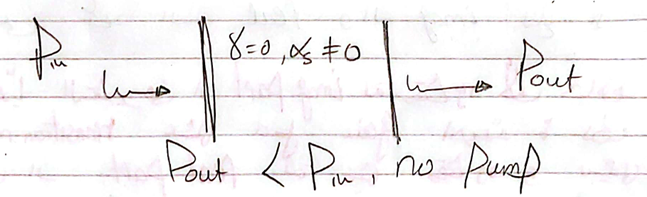
\includegraphics[scale=0.8]{1.png}
\end{center}
The propagation constant is $\beta$ (no additional $\Delta \beta$), so the resonance condition is:
\begin{align*}
    \beta L &= q \pi  \\
    \nu_q &= \frac{qc}{2L} = q \nu_F
\end{align*}

\subsubsection{Active Cavities}
In active cavities, there is a pump and amplification, so $\gamma \neq 0$ and $\alpha_s \neq 0$.
\begin{center}
    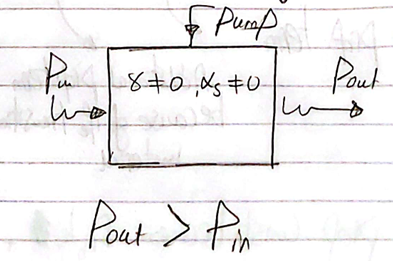
\includegraphics[scale=0.8]{2.png}
\end{center}
The propagation constant is $\beta + \Delta \beta$, so the resonance condition is:
\begin{align*}
    (\beta + \Delta \beta) L &= q \pi
\end{align*}
$\beta = \frac{2 \pi}{\lambda}$ and $\Delta \beta = \frac{(\nu - \nu_o) \gamma}{\Delta \nu}$, so:
\begin{align*}
    \frac{2 \pi \nu}{c} L + \frac{(\nu - \nu_o) \gamma}{\Delta \nu} L &= q \pi
\end{align*}
Multuplying by $\frac{c}{2 \pi L}$:
\begin{align*}
    \nu + \frac{(\nu - \nu_o) \gamma}{\Delta \nu} L \frac{c}{2 \pi L} &= q \pi \frac{c}{2 \pi L} \\
    \nu + \frac{(\nu - \nu_o) \gamma}{\Delta \nu} \frac{c}{2 \pi} &= q \nu_F
\end{align*}
So:
\begin{align*}
    \nu_{res_{new}} = \nu_{res_{old}} - \frac{(\nu - \nu_o) \gamma}{\Delta \nu} \frac{c}{2 \pi}
\end{align*}
$\nu_o$ pulls the resonance frequency towards itself, so if:
\begin{itemize}
    \item $\nu - \nu_o < 0 \rightarrow \nu_{res_{new}} > \nu_{res_{old}}$
    \item $\nu - \nu_o > 0 \rightarrow \nu_{res_{new}} < \nu_{res_{old}}$
    \item $\nu - \nu_o = 0 \rightarrow \nu_{res_{new}} = \nu_{res_{old}}$
\end{itemize}
\begin{align*}
    \nu_q = q \nu_F = \nu + \frac{(\nu - \nu_o) \gamma}{\Delta \nu} \frac{c}{2 \pi}
\end{align*}
To draw $\nu_{res_{old}}$ vs $\nu_{res_{new}}$, we will use superposition:
\begin{itemize}
    \item $\nu_q = \nu$
    \item $\nu_q = \frac{(\nu - \nu_o) \gamma}{\Delta \nu} \frac{c}{2 \pi} \rightarrow$ this relation decays when moving away from the $\nu_o$ because of $\gamma$
\end{itemize}
\begin{center}
    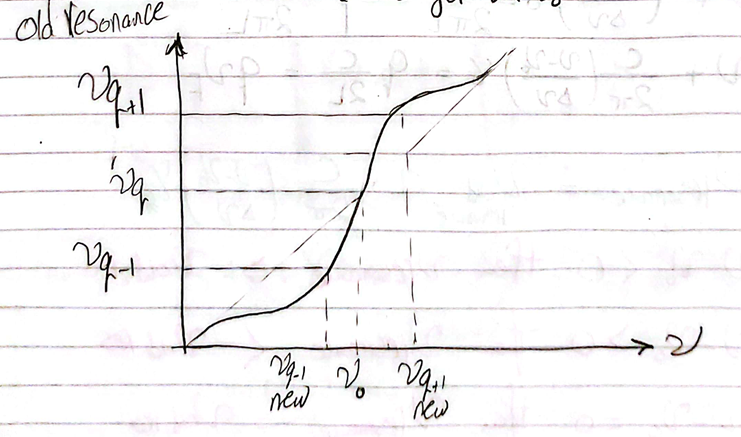
\includegraphics[scale=0.8]{3.png}
\end{center}
Frequency pulling is a problem in intensity modulation, where we use different pump currents producing different gains to modulate data, but unintentionally change the resonance frequency.

\section{Radiative Scattering in Semiconductors}
\begin{itemize}
    \item \textbf{Emission:} An electron moves from the conduction band to the valence band, emitting a photon.
    \item \textbf{Absorption:} An electron absorbs a photon and moves from the valence band to the conduction band.
    \item We need to apply the conservation of energy and momentum for both processes. 
    \item Recall that $\vec{P} = \hbar \vec{k}$ or $P = \hbar k = \frac{\hbar 2 \pi}{\lambda} = \frac{h}{\lambda}$.
\end{itemize}

\subsection{Emission}
\begin{itemize}
    \item \textbf{Before the collision:} There is an electron in $E_2$
    \item \textbf{After the collision:} The electron moves to $E_1$ and emits a photon.
\end{itemize}
\begin{align*}
    E_2 &= E_1 + E_{ph} \\
    \hbar \vec{k}_2 &= \hbar \vec{k}_1 + \hbar \vec{k}_{ph}
\end{align*}
In solids, the wavefunction of the electron has a wavelength in the order of the lattice constant (angstroms),  while the photon has a wavelength in the order of the micron. So, the electron's momentum is much higher than the photon's momentum, so we neglect the photon's momentum:
\begin{align*}
    \vec{k}_2 &= \vec{k}_1 + \vec{k}_{ph} \approx \vec{k}_1
\end{align*}
So in order to get radiative interaction, the electron must move from a state with a certain momentum to a state with the same momentum. This is called \textbf{momentum conservation}.
\begin{center}
    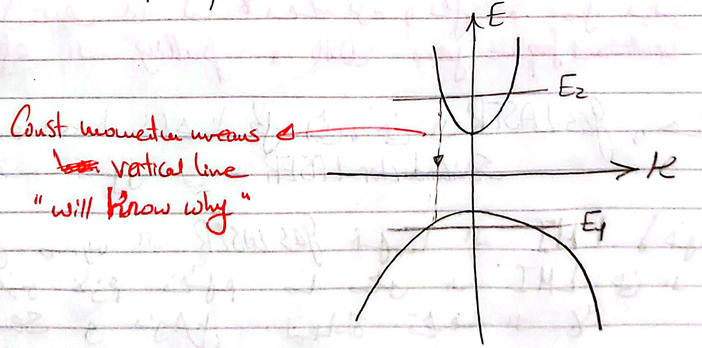
\includegraphics[scale=0.7]{4.png}
\end{center}
\textbf{Note:} There might be a non-radiative interaction if the momentum of the states are different.

\subsection{Absorption}
\begin{itemize}
    \item \textbf{Before the collision:} There is an electron in $E_1$ and a photon.
    \item \textbf{After the collision:} The electron moves to $E_2$.
\end{itemize}
\begin{align*}
    E_1 + E_{ph} &= E_2 \\
    \hbar \vec{k}_1 + \hbar \vec{k}_{ph} &= \hbar \vec{k}_2
\end{align*}
$\hbar \vec{k}_1 >> \hbar \vec{k}_{ph}$, so:
\begin{align*}
    \vec{k}_1 &\approx \vec{k}_2
\end{align*}

\subsection{Direct \& Indirect Gap Materials}
\begin{center}
    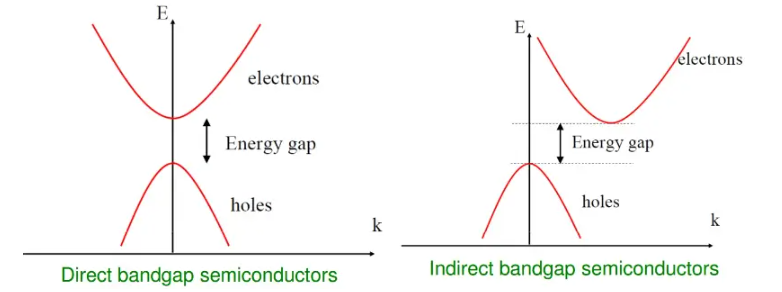
\includegraphics[scale=0.7]{5.png}
\end{center}
\begin{itemize}
    \item \textbf{Direct Gap Materials:} The minimum energy of the conduction band and the maximum energy of the valence band are at the same momentum. So, the electron can move from the conduction band to the valence band without changing its momentum. This is the case for GaAs.
    \item \textbf{Indirect Gap Materials:} The minimum energy of the conduction band and the maximum energy of the valence band are at different momenta. So, the electron must change its momentum to move from the conduction band to the valence band. This is the case for Si.
    \item Changing the momentum (moving horizontally in the band diagram) is called Phonon Scattering. Having both phonon and photon scattering is called Phonon-Assisted Emission.
    \item In phonon scattering, photons have a very large frequency do its momentum can't be neglected, but they have negligible energy, so: $E_2 \approx E_1$ and $\vec{k}_2 =\vec{k}_1 + \vec{k}_{ph}$.
\end{itemize}
There are many scattering mechanisms in semiconductors (not just radiative scattering), so we define a prameter called internal quantum efficiency ($\eta_{int}$) to measure the ratio of radiative scattering to all scattering mechanisms:
\begin{align*}
    \eta_{int} = \frac{\frac{1}{\tau_r}}{\frac{1}{\tau}} \text{ where } \tau = \tau_r + \tau_{nr}
\end{align*}
In direct gap materials such as GaAs, $\eta_{int} \approx \frac{1}{2}$, while in indirect gap materials such as Si, $\eta_{int} \approx \frac{1}{10,000}$.

\subsection{Optical Joint Density of States $\rho_j(\nu)$}
\begin{itemize}
    \item From the previous section, in order to have interaction, we must have 2 states with the same momentum. This is called the k-selection rule.
    \item Every $E_c$ state has a corresponding $E_v$ state that has the same momentum, and the output photon has energy equal to the difference between the two states.
    \item We can relate $E_1$, $E_2$, $k$ and $h\nu$
\end{itemize}
Recall that $E = P.E + K.E$:
\begin{align}
    E_2 = E_c + \frac{\hbar^2 k^2}{2 m_e} \\
    E_1 = E_v - \frac{\hbar^2 k^2}{2 m_h} \notag
\end{align}
So:
\begin{align*}
    h \nu &= E_2 - E_1 = E_c + \frac{\hbar^2 k^2}{2 m_e} - E_v + \frac{\hbar^2 k^2}{2 m_h} \\
    &= E_g + \frac{\hbar^2 k^2}{2} \left(\frac{1}{m_e} + \frac{1}{m_h}\right) = E_g + \frac{\hbar^2 k^2}{2 m_r} 
\end{align*}
where $m_r$ is the reduced effective mass \& $\frac{1}{m_r} = \frac{1}{m_e} + \frac{1}{m_h}$
\begin{align*}
    \frac{\hbar^2 k^2}{2} = m_r (h \nu - E_g)
\end{align*}
From (1)
\begin{align*}
    E_2 &= E_c + \frac{m_r}{m_e} (h \nu - E_g) \\
    dE_2 &= \frac{m_r}{m_e} d \nu
\end{align*}
The number of states within $\Delta E$ in the conduction band is equal to the number of states in the valence band within a $\Delta E$ which contains the same $\Delta k$ in the conduction band. So:
\begin{align*}
    \int_{\Delta E_c} S_c(E) \, dE = \int_{\Delta E_v} S_v(E) \, dE
\end{align*}
Note that $\Delta E_c \neq \Delta E_v$, but they include levels with the same $\Delta k$ according to the k-rule.
\begin{center}
    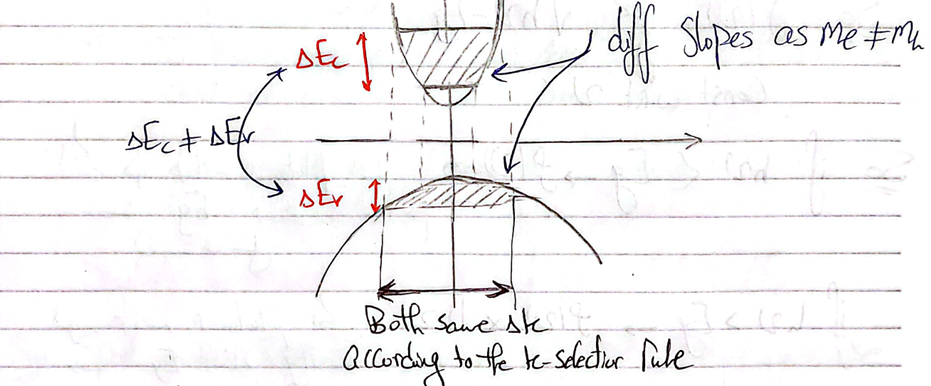
\includegraphics[scale=0.7]{6.png}
\end{center}
For the photon to interact, there must be available states in the conduction AND valence bands, so:
\begin{align*}
    \text{\# photons that may interact} = \text{\# states in conduction band} = \text{\# states in valence band}
\end{align*}
We have a direct relation between $E_1$ and $\nu$, thus saying $\rho(\nu)$ doesn't differ from $\rho(E)$, but we usually define the $\rho$ by frequency:
\begin{align*}
    \rho(\nu) d\nu &= S_c(E_2) dE_2 \\
    \rho(\nu) &= S_c(E_2) \frac{dE_2}{d\nu} = S_c(E_2) \frac{h m_r}{m_e} \\
    &= \text{const} \sqrt{E_2 - E_c} = \text{const} \sqrt{h \nu - E_g}
\end{align*}
So:\begin{align*}
    \rho(\nu) = B \sqrt{h \nu - E_g}, \text{ where B is a constant w.r.t. $\nu$}
\end{align*}
\begin{itemize}
    \item If $h \nu < E_g \rightarrow \rho(\nu) = 0$ (No interaction if $E_{ph} < E_g$)
    \item If $h \nu > E_g \rightarrow \rho(\nu) \propto \sqrt{h \nu}$
\end{itemize}
\begin{center}
    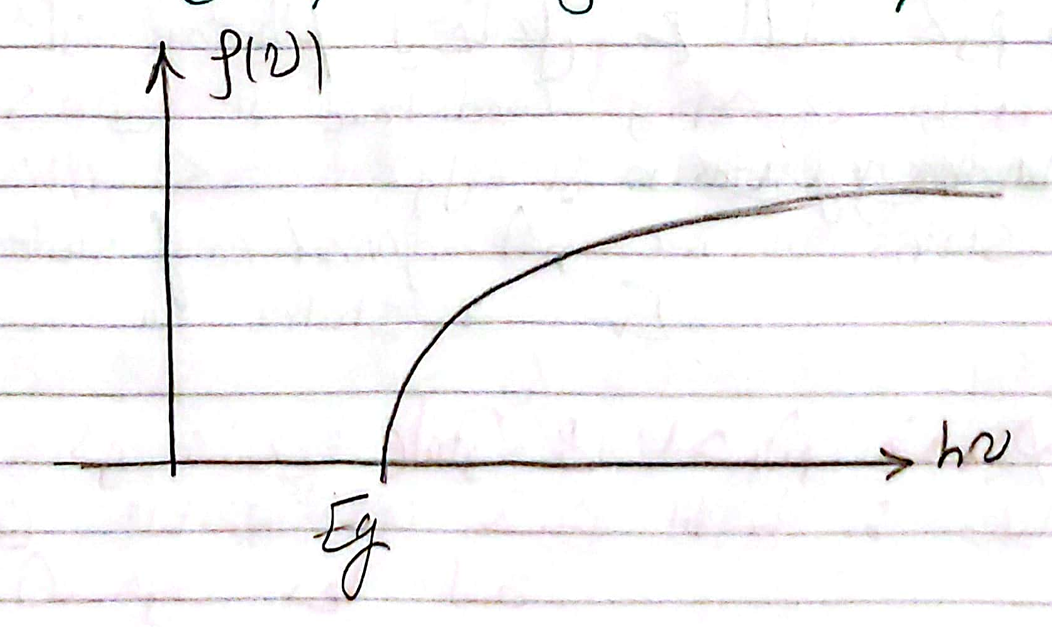
\includegraphics[scale=0.45]{7.png}
\end{center}

\section{Gain in Semiconductors}
To get number of emissions and absorptions:
\begin{enumerate}
    \item \textbf{Transition rates} (same as gas LASER)
    \item \textbf{Occupancy probability:} The probability of having an electron in the conduction band and a hole in the valence band.
    \item \textbf{Optical joint density of states:} The number of states in the conduction band that can interact with the valence band.
\end{enumerate}
From occupancy probability, the probability of emission:
\begin{align*}
    f_e (\nu) = f_c (E_2) [1 - f_v (E_1)]
\end{align*}
Similarly, the probability of absorption:
\begin{align*}
    f_a (\nu) = [1 - f_c (E_2)] f_v (E_1)
\end{align*}
So:
\begin{itemize}
    \item \textbf{Spontaneous Emission Rate:} $r_{sp} = \frac{1}{\tau_r} f_c(\nu) \rho_j (\nu)$
    \item \textbf{Stimulated Emission Rate:} $r_{st} = \sigma \phi_{\nu} f_e (\nu) \rho_j (\nu)$
    \item \textbf{Absorption Rate:} $r_{ab} = \sigma \phi_{\nu} f_a (\nu) \rho_j (\nu)$
\end{itemize}
Note that the Fermi-Dirac distribution is a statistical function that describes the probability of a quantum state being occupied by aan electron at a given energy and temperature. 
\begin{align*}
    f_c = \frac{1}{1 + e^{\frac{E_c - E_{f_c}}{kT}}} \text{ and } f_v = \frac{1}{1 + e^{\frac{E_v - E_{f_v}}{kT}}}
\end{align*}
where $E_{f_c} = E_{f_v} = E_f$ at thermal equilibrium. \\ \\
To get the gain, we assume we have a sample of length $\Delta z$ and area $A$, the input is $\phi_\nu (z)$ and the output is $\phi_\nu (z + \Delta z)$. We will neglect the spontaneous emission rate:
\begin{align*}
    \phi_\nu (z + \Delta z) A = \phi_\nu (z) A + \Delta z A (r_{st} - r_{ab}) \\
    \phi_\nu (z + \Delta z) - \phi_\nu (z) = \Delta z (r_{st} - r_{ab})
\end{align*}
So:
\begin{align*}
    \frac{d\phi_\nu}{\Delta z} = r_{st} - r_{ab} = \sigma \phi_\nu (f_e(\nu) - f_a(\nu)) \rho_j (\nu) = \gamma \phi_\nu
\end{align*}
where $\gamma = \sigma (f_e(\nu) - f_a(\nu)) \rho_j (\nu)$ is the gain coefficient.
\begin{align*}
    f_e(\nu) - f_a(\nu) &= f_c(E_2) [1 - f_v(E_1)] - [1 - f_c(E_2)] f_v(E_1) \\
    &= f_c(E_2) - f_c(E_2) f_v(E_1) - f_v(E_1) + f_c(E_2) f_v(E_1) \\
    &= f_c(E_2) - f_v(E_1) 
\end{align*}
So:
\begin{align*}
    \gamma = \sigma \rho_j (\nu) [f_c(E_2) - f_v(E_1)] = \sigma \rho_j (\nu) f_g (\nu)
\end{align*}
where $f_g (\nu)$ is the fermi inversion factor, and it is similar to $N_2-N_1$ in gas LASERs. 

\subsection{Lineshape Function}
\begin{itemize}
    \item In gases, there are energy levels, so the uncertainity is that you don't know the exact energy of the level ($E + \Delta E$). 
    \item However, in semiconductors, there are energy bands not levels, so $\Delta E$ is the range of energies that have the same momentum. The uncertainity here is that you cannot know the exact momentum and energy of the electron at the same time.
    \item If we are certain about the momentum from the k-selection rule, there is $\Delta E$ in the band that can satisfy the k-selection rule.
    \item The result of this uncertainity is that for a certain momentum ($k$), we have many frequencies that can satisfy the k-selection rule. This is called the \textbf{Lineshape Function}.
    \item To get the rate (number of electrons that can interact with the photon per unit time per unit volume), we need to integrate over all possible frequencies.
\end{itemize}
$\sigma = \frac{\lambda^2}{8 \pi \tau_r} g_{\nu_o}(\nu)$:
\begin{align*}
    r_{st} = \int_{-\infty}^{\infty} \frac{\lambda^2}{8 \pi \tau_r} \phi_\nu f_e (\nu) \rho_j (\nu) g_{\nu_o}(\nu) \, d\nu
\end{align*}
But the $\sqrt{E}$ dependency in $\rho_j (\nu)$ is much slower than $g_{\nu_o}(\nu)$, so we can approximate $g_{\nu_o}(\nu)$ by a delta function, so the $\rho_j (\nu)$ is sampled at the center frequency:
\begin{align*}
    r_{st} = \frac{\lambda^2}{8 \pi \tau_r} \phi_{\nu} f_e (\nu) \rho_j (\nu)
\end{align*}
So:
\begin{align*}
    \gamma = \frac{\lambda^2}{8 \pi \tau_r} \rho_j (\nu) f_g (\nu)
\end{align*}
\begin{itemize}
    \item The first term $\frac{\lambda^2}{8 \pi \tau_r}$ is approximately constant with frequency.
    \item The second term $\rho_j (\nu)$ is always positive and has a $\sqrt{E}$ dependency.
    \item The third term $f_g (\nu) = f_c(E_2) - f_v(E_1)$ can be positive or negative.
\end{itemize}
\pagebreak
\textbf{Case A: At Thermal Equilibrium ($E_{f_c} = E_{f_v} = E_f$)}
\begin{center}
    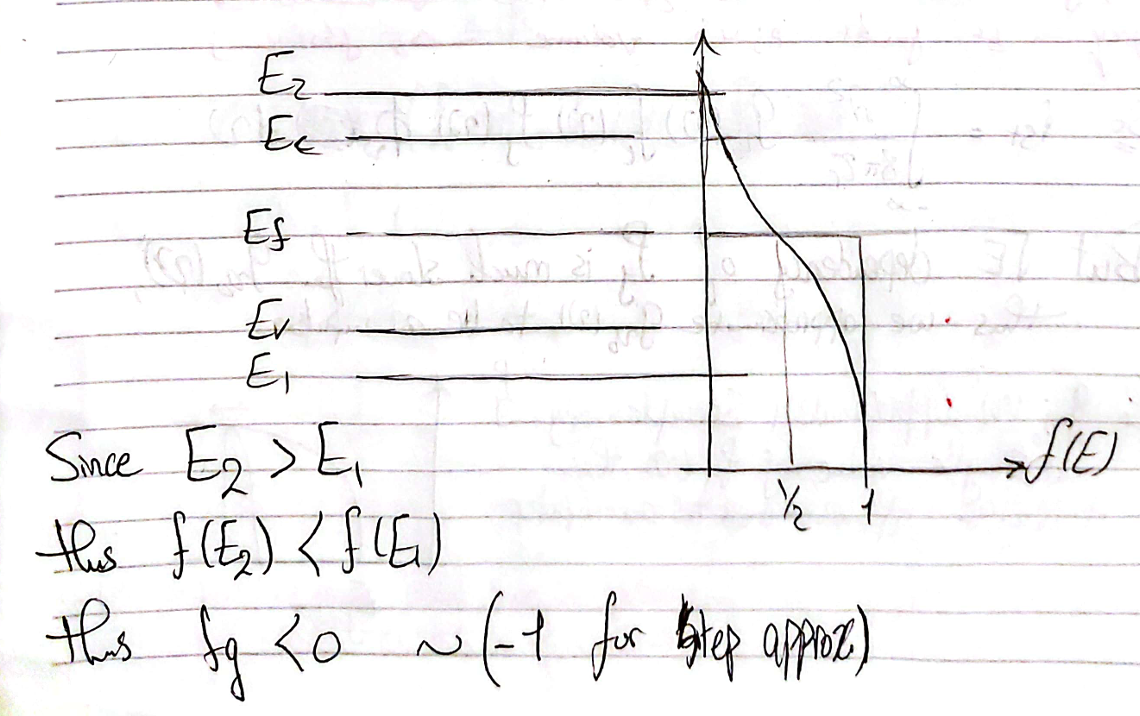
\includegraphics[scale=0.6]{8.png}
\end{center}
\textbf{Case B: Non-Degenerate Case ($E_{f_c} \neq E_{f_v}$)}
\begin{center}
    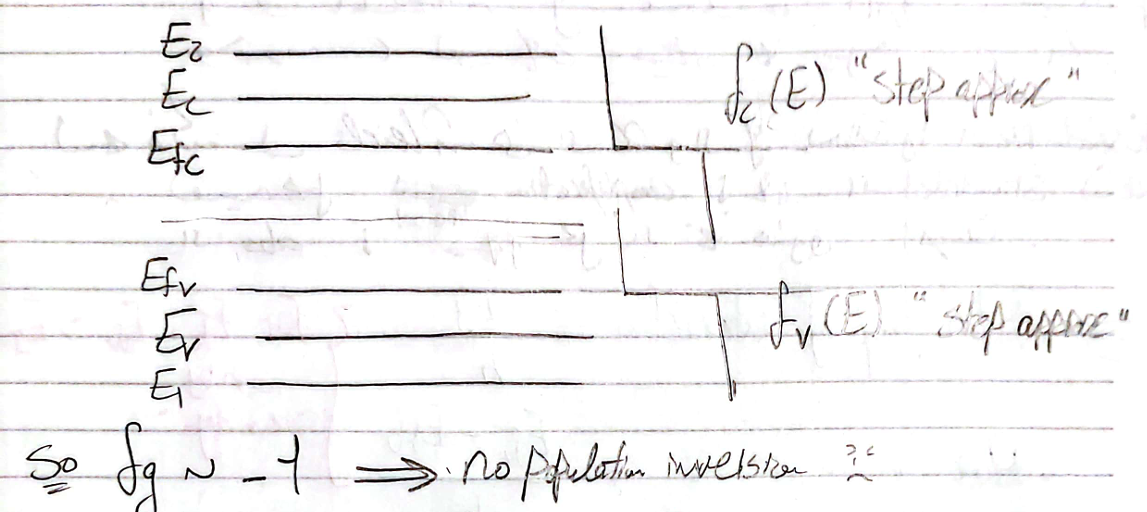
\includegraphics[scale=0.6]{9.png}
\end{center}
\textbf{Case C: Degenerate Case ($E_{f_c} > E_c$ and $E_{f_v} < E_v$)}
\begin{center}
    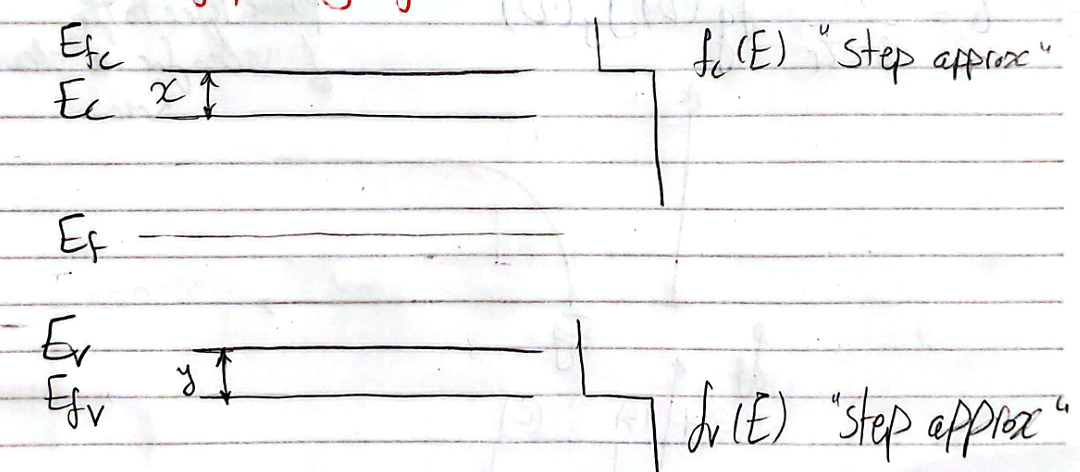
\includegraphics[scale=0.6]{10.png}
\end{center}
\begin{itemize}
    \item If $E_2$ is found in the $x$ region AND $E_1$ is found in the $y$ region, then $f_g (\nu) = 1 - 0 = 1$ (positive), so we have population inversion.
    \item In region $x$, $f_c = 1$ so electron presence probability is 100\% (no holes), while in region $y$, $f_v = 0$ so electron presence probability is 0\% (no electrons). So any 2 levels in the $x$ region and $y$ region that satisfy the k-selection rule will lead to amplification as stimulated is greater than absorption since all electrons are in the conduction band.
\end{itemize}
For degenerate only:
\begin{itemize}
    \item Minimum interaction frequency is $\frac{E_g}{h}$
    \item Maximum interaction frequency is $\frac{E_{f_c} - E_{f_v}}{h}$
\end{itemize}
\begin{center}
    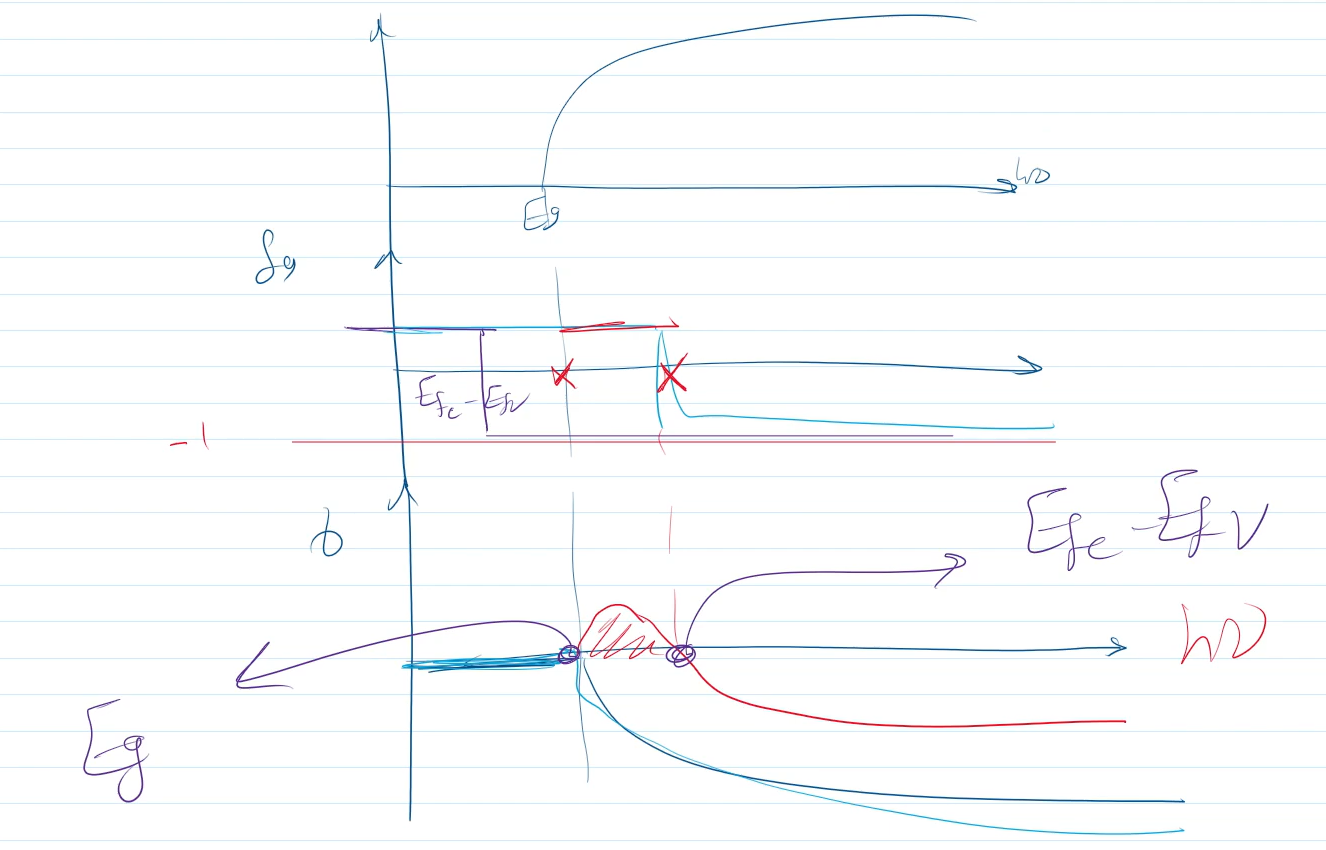
\includegraphics[scale=0.6]{11.png}
\end{center}


\end{document}